%************************************************
\chapter{Column Chromatography}
%************************************************
\begin{flushright}
February 11, 2013
\end{flushright}
\section{Aim}
To separate a given mixture of 2 colourless compounds, using the Column Chromatography technique, viz. Benzophenone and Bipyridine.

\section {Chemicals Required}
	\begin{enumerate}
		\item Silica
		\item Iodine
		\item Ethyl Acetate
		\item Benzene
		\item Benzophenone (given compound, refer to \autoref{e4_compound1})
		\item Bipyridine (given compound, refer to \autoref{e4_compound2})
	\end{enumerate}

	\begin{figure}[bth]
		\begin{center}
			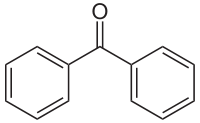
\includegraphics[width=0.4\linewidth]{gfx/e4_compound1}
		\end{center}
	\caption[Benzophenone]{\label{e4_compound1}}
	\end{figure}

	\begin{figure}[bth]
		\begin{center}
			
\includegraphics[width=0.4\linewidth]{gfx/e4_compound2}
		\end{center}
	\caption[Bipyridine]{\label{e4_compound2}}
	\end{figure}

\section{Theory}
	The theory for this experiment is the same as that of the previous experiment, with specifically, the only difference being the use of colourless compounds in this experiment.
	\par
	For easy reference, the theory of the previous experiment has been replicated here. \\
	TLC is good for detecting what constitutes a mixture. However its yield is very little. To overcome this difficulty, we use a technique known as ``Column Chromatography''. The principle of differential binding of compounds with the solvent is still harnessed. However, instead of relying on the capillary action, we now rely on gravity. The setup consists of a vertical wet (hexane) silica column, contained in a suitable glass container with a flow control apparatus and a nozzle at the bottom. The compound (if solid, then first dissolved in an appropriate solvent) is added on top of the silica column and on top of it the eluent (a suitably polar solution) is added. This moves down through the silica column, differentially moving the constituents of the mixture (which is just a compound in our case). Then if the compound is visible, we can easily use this property and collect the constituents in different test tubes. However, if the compounds are not visible, we may need to run a TLC for each small volume collected.
	\par
	Wikipedia has a very concise and accurate description of the same, which can also be referred to.


\section{Procedure}	
	\begin{enumerate}
		\item Determining the concentration of Elluent to use
		\begin{enumerate}
			\item Prepared the TLC plates as in the previous experiments
			\item Setup the Visibility Chamber, again as before
			\item Created a $10\%$ Ethyl Acetate Soln. in Hexane
			\item The given compounds were dissolved suitably in Ethyl Acetate.
			\item TLC was run using the given compounds, with Benzophenone on the left, co-spot in the centre, and Bipyridine in the right.
			\item Since the compounds' $R_f$ values were satisfactory in this concentration, the experiment was carried out with an Elluent of $10\%$ EtAc concentration. Refer to \autoref{e4_1} for details.
		\end{enumerate}
		\item Preparing the Wet Column (same as before, replicated here for convenience)
		\begin{enumerate}
			\item While the TLCs run, a slurry of silica was created in hexane (with about 20-30 spatula of silica) and it was poured in glass column, as described in the theory.
			\item To this, hexane was added, and it was shaken until all air bubbles disappeared. Further the volume of hexane was reduced to about $1$ cm above the silica gel alongside, by allowing hexane to flow through the nozzle.
			\item The compound, along with silica, were mixed with ethyl acetate to form a thick slurry.
			\item This mixture was transferred on top of the silica column.
			\item After it settled reasonably, cotton was added to further level and to ensure that addition of elluent doesn't disturb the mixture (in this case the compound). This ensures that when the separation process proceeds, it doesn't happen out of plane (with respect to the cross section of the container)
		\end{enumerate}
		\item Running the Column (the first three points are the same as before)
		\begin{enumerate}
			\item Got a set of ordered test tubes in a suitable holder.
			\item The Elluent was poured into the glass column cautiously and sealed from the top.
			\item The liquid was allowed to flow through the nozzle of the glass column, into the test tubes, progressively, as they filled.
			\item After the first test tube, a sample from two test-tubes was run on a single TLC to determine the compounds present.
			\item The concentration of the Elluent was increased once the first compound was recovered successfully.
		\end{enumerate}


	\end{enumerate}
\section{Observations and Results}		
	To find the concentration of Elluent to use, we ran the TLCs as required. For details, please refer to \autoref{e4_1}. We used a $10\%$ EtAc solution, with the following $R_f$ values from the first run:
	\begin{enumerate}
		\item Bipyridine $R_f$ = 0.202
		\item Benzophenone $R_f$=0.833
	\end{enumerate}
	and from the second run
	\begin{enumerate}
		\item Bipyridine $R_f$ = 0.289
		\item Benzophenone $R_f$=0.789
	\end{enumerate}
	\par
	We ran the column for about 38 test tubes, and ran TLC for 32 of them. $R_f$ values for individual tubes were not calculated as they were clearly for the compounds in question. Following is a list of test tubes in which the compounds were found. Details for the same are given in \autoref{e4_1} and \autoref{e4_2}.
	\par
	NOTE: The starting point of the TLC is at the top for most slides shown in the image.
	\begin{enumerate}
		\item Benzophenone: Test tube 5 and 6
		\item Bipyridine: Test Tube 19 to 28
	\end{enumerate}
	The mixture was eventually separated into its constituents, as given shown in \autoref{e4_3}.

\section{Precaution}
	Precautions are same as those in the previous experiment (except the last), viz.
	\begin{enumerate}
		\item The slurry shouldn't be very thick
		\item Cover the beakers with a watch glass to ensure there's no loss of volatile substances (minimal that is)
		\item The coating is very fragile, thus the TLC plates must be handled with caution
		\item We've to ensure there aren't any air bubbles in the column created, by tapping it enough.
		\item The hexane level shouldn't drop below the silica column's top, else cracks would begin to appear.
		\item Ensure the test tubes aren't cracked.
		\item If the elluent level rises into the funnel, do not remove the funnel. The air-pressure causes oscillations to setup and the elluent doesn't overflow (assuming the funnel is in complete contact with the column).
	\end{enumerate}

	
\section{Acknowledgements}
I thank Dr. R Vijaya Anand for his guidance during the experiment. I also acknowledge the contribution of my lab partners, Vivek, Prashansa and Srijit for performance of the same. I also thank our PhD guide for demonstrating the experiment and her assistance in general, with performance of the same.

	\clearpage
	\begin{figure}[bth]
		\begin{center}
			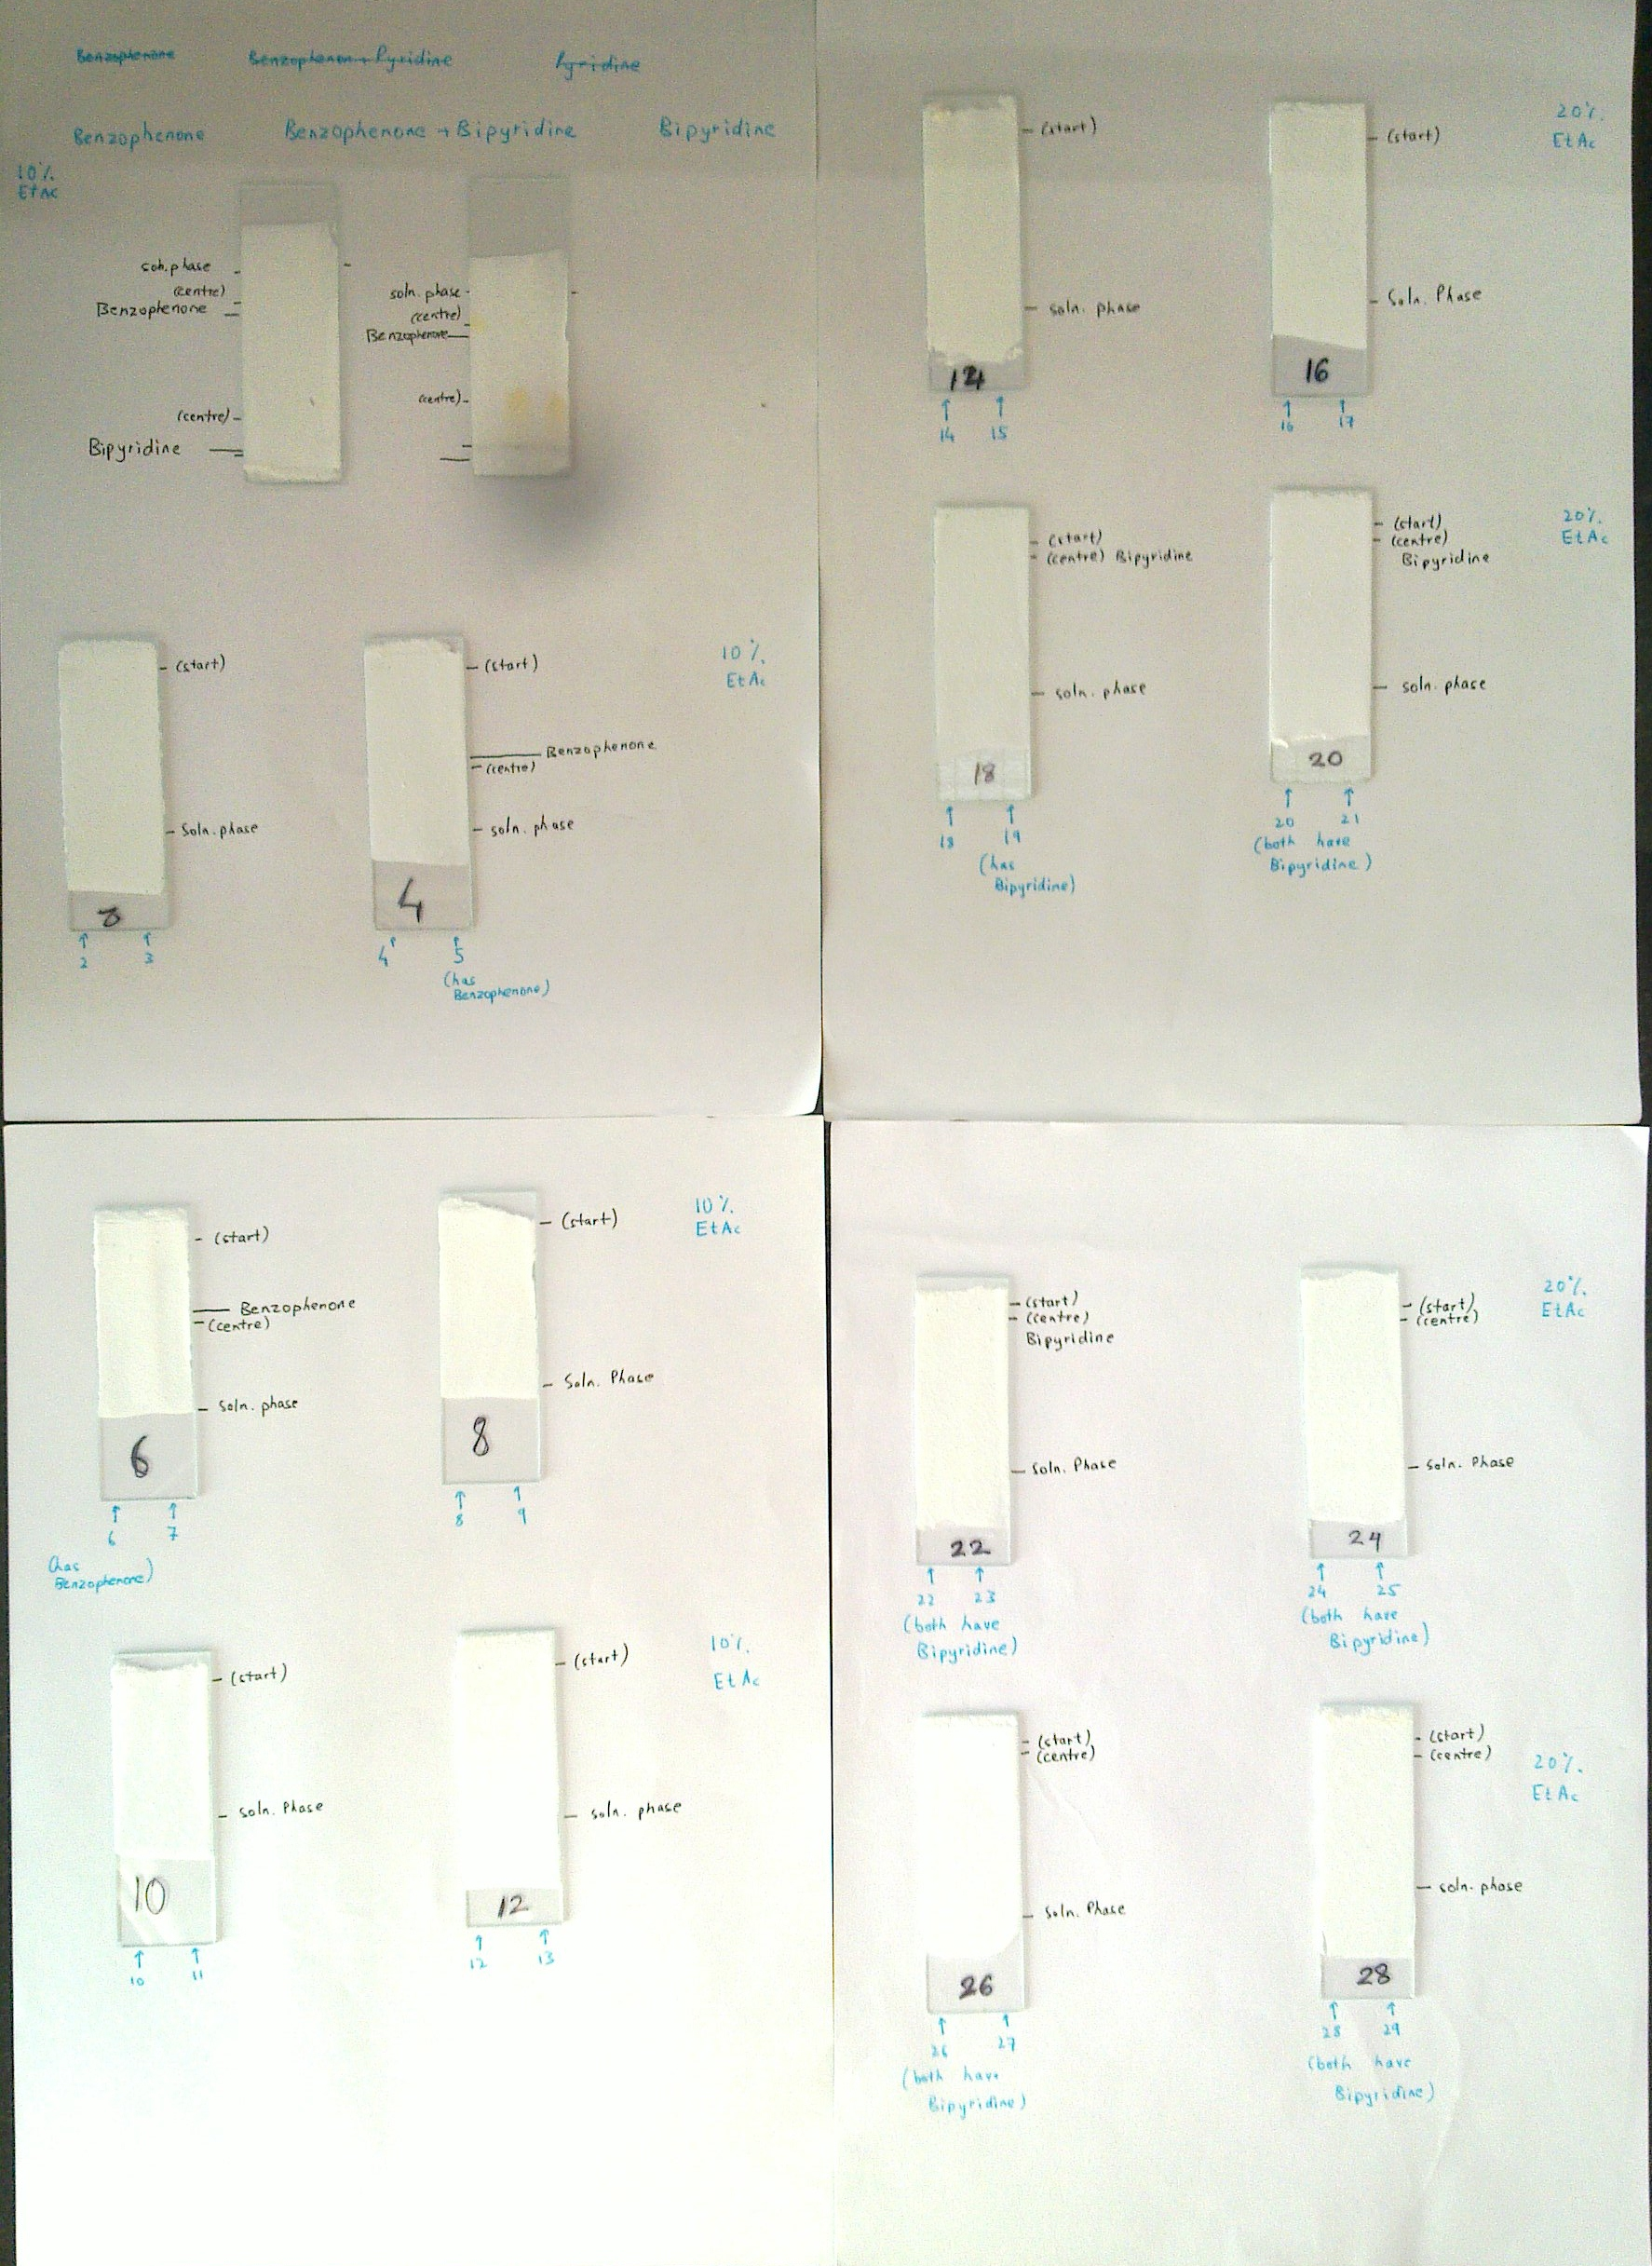
\includegraphics[width=1.5\linewidth]{gfx/e4_1}
		\end{center}
	\caption[TLCs Set 1]{\label{e4_1}}
	\end{figure}

	\begin{figure}[bth]
		\begin{center}
			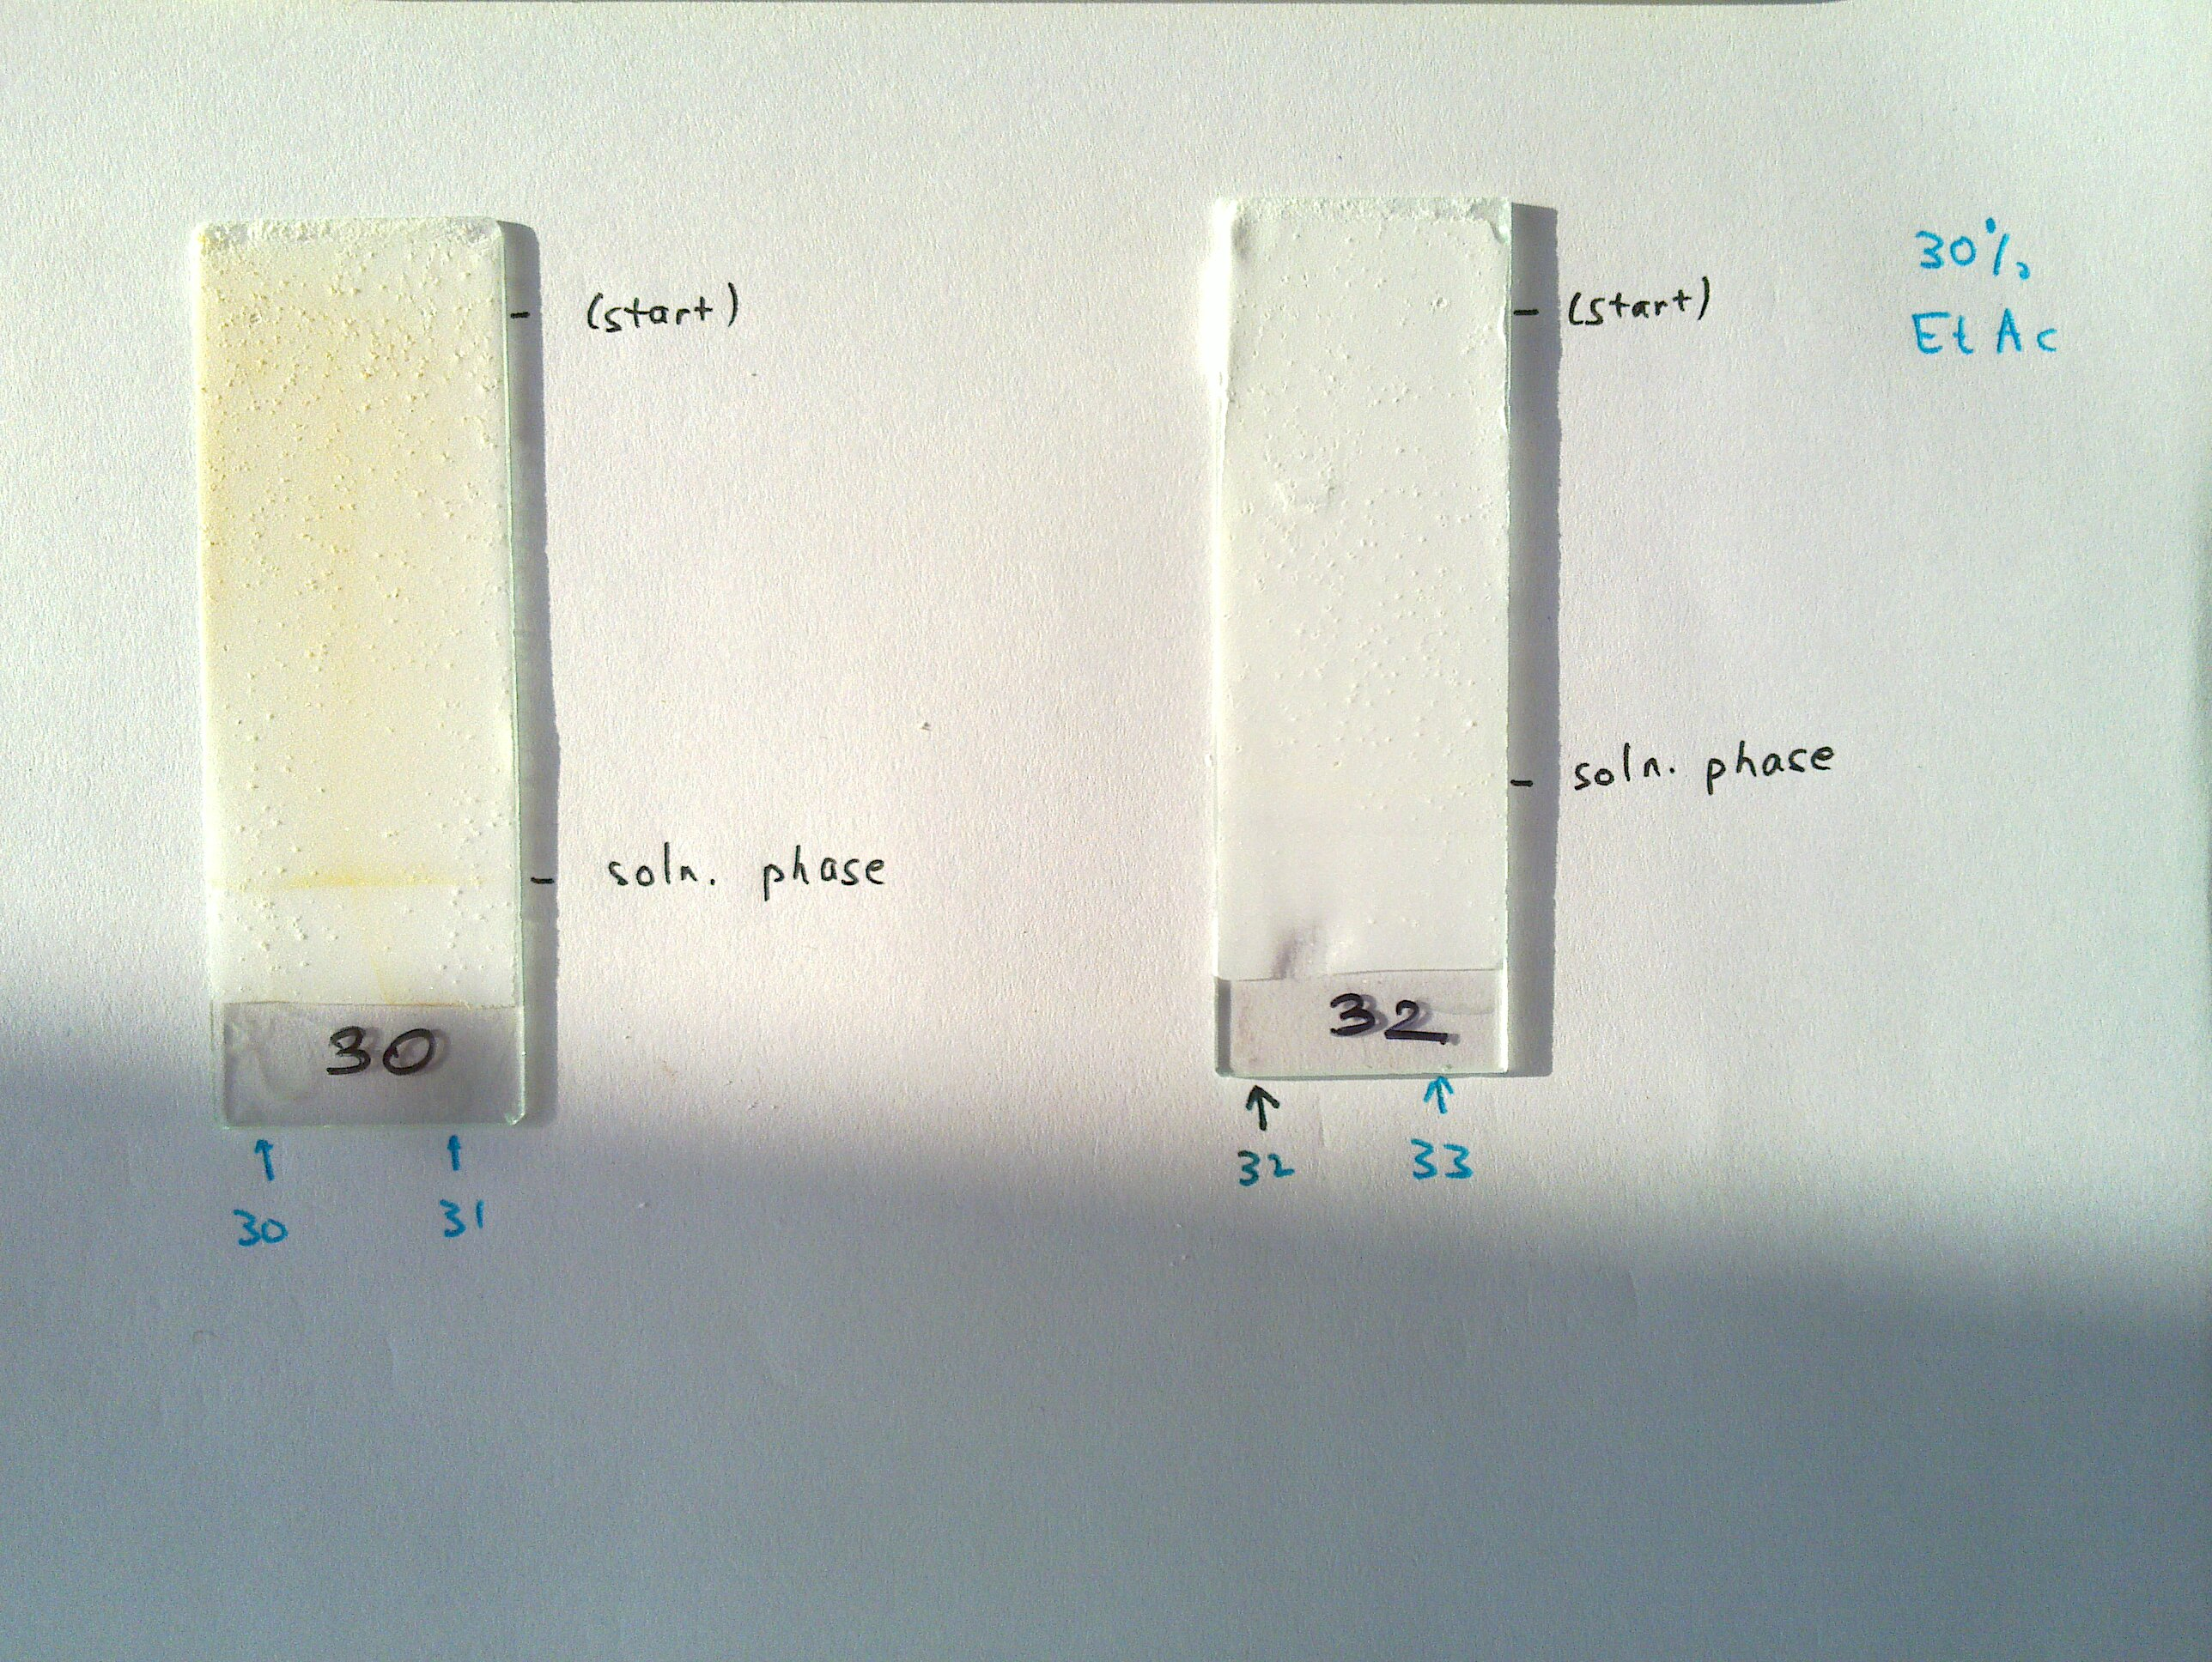
\includegraphics[width=0.6\linewidth]{gfx/e4_2}
		\end{center}
	\caption[TLCs Set 2]{\label{e4_2}}
	\end{figure}


	\begin{figure}[bth]
		\begin{center}
			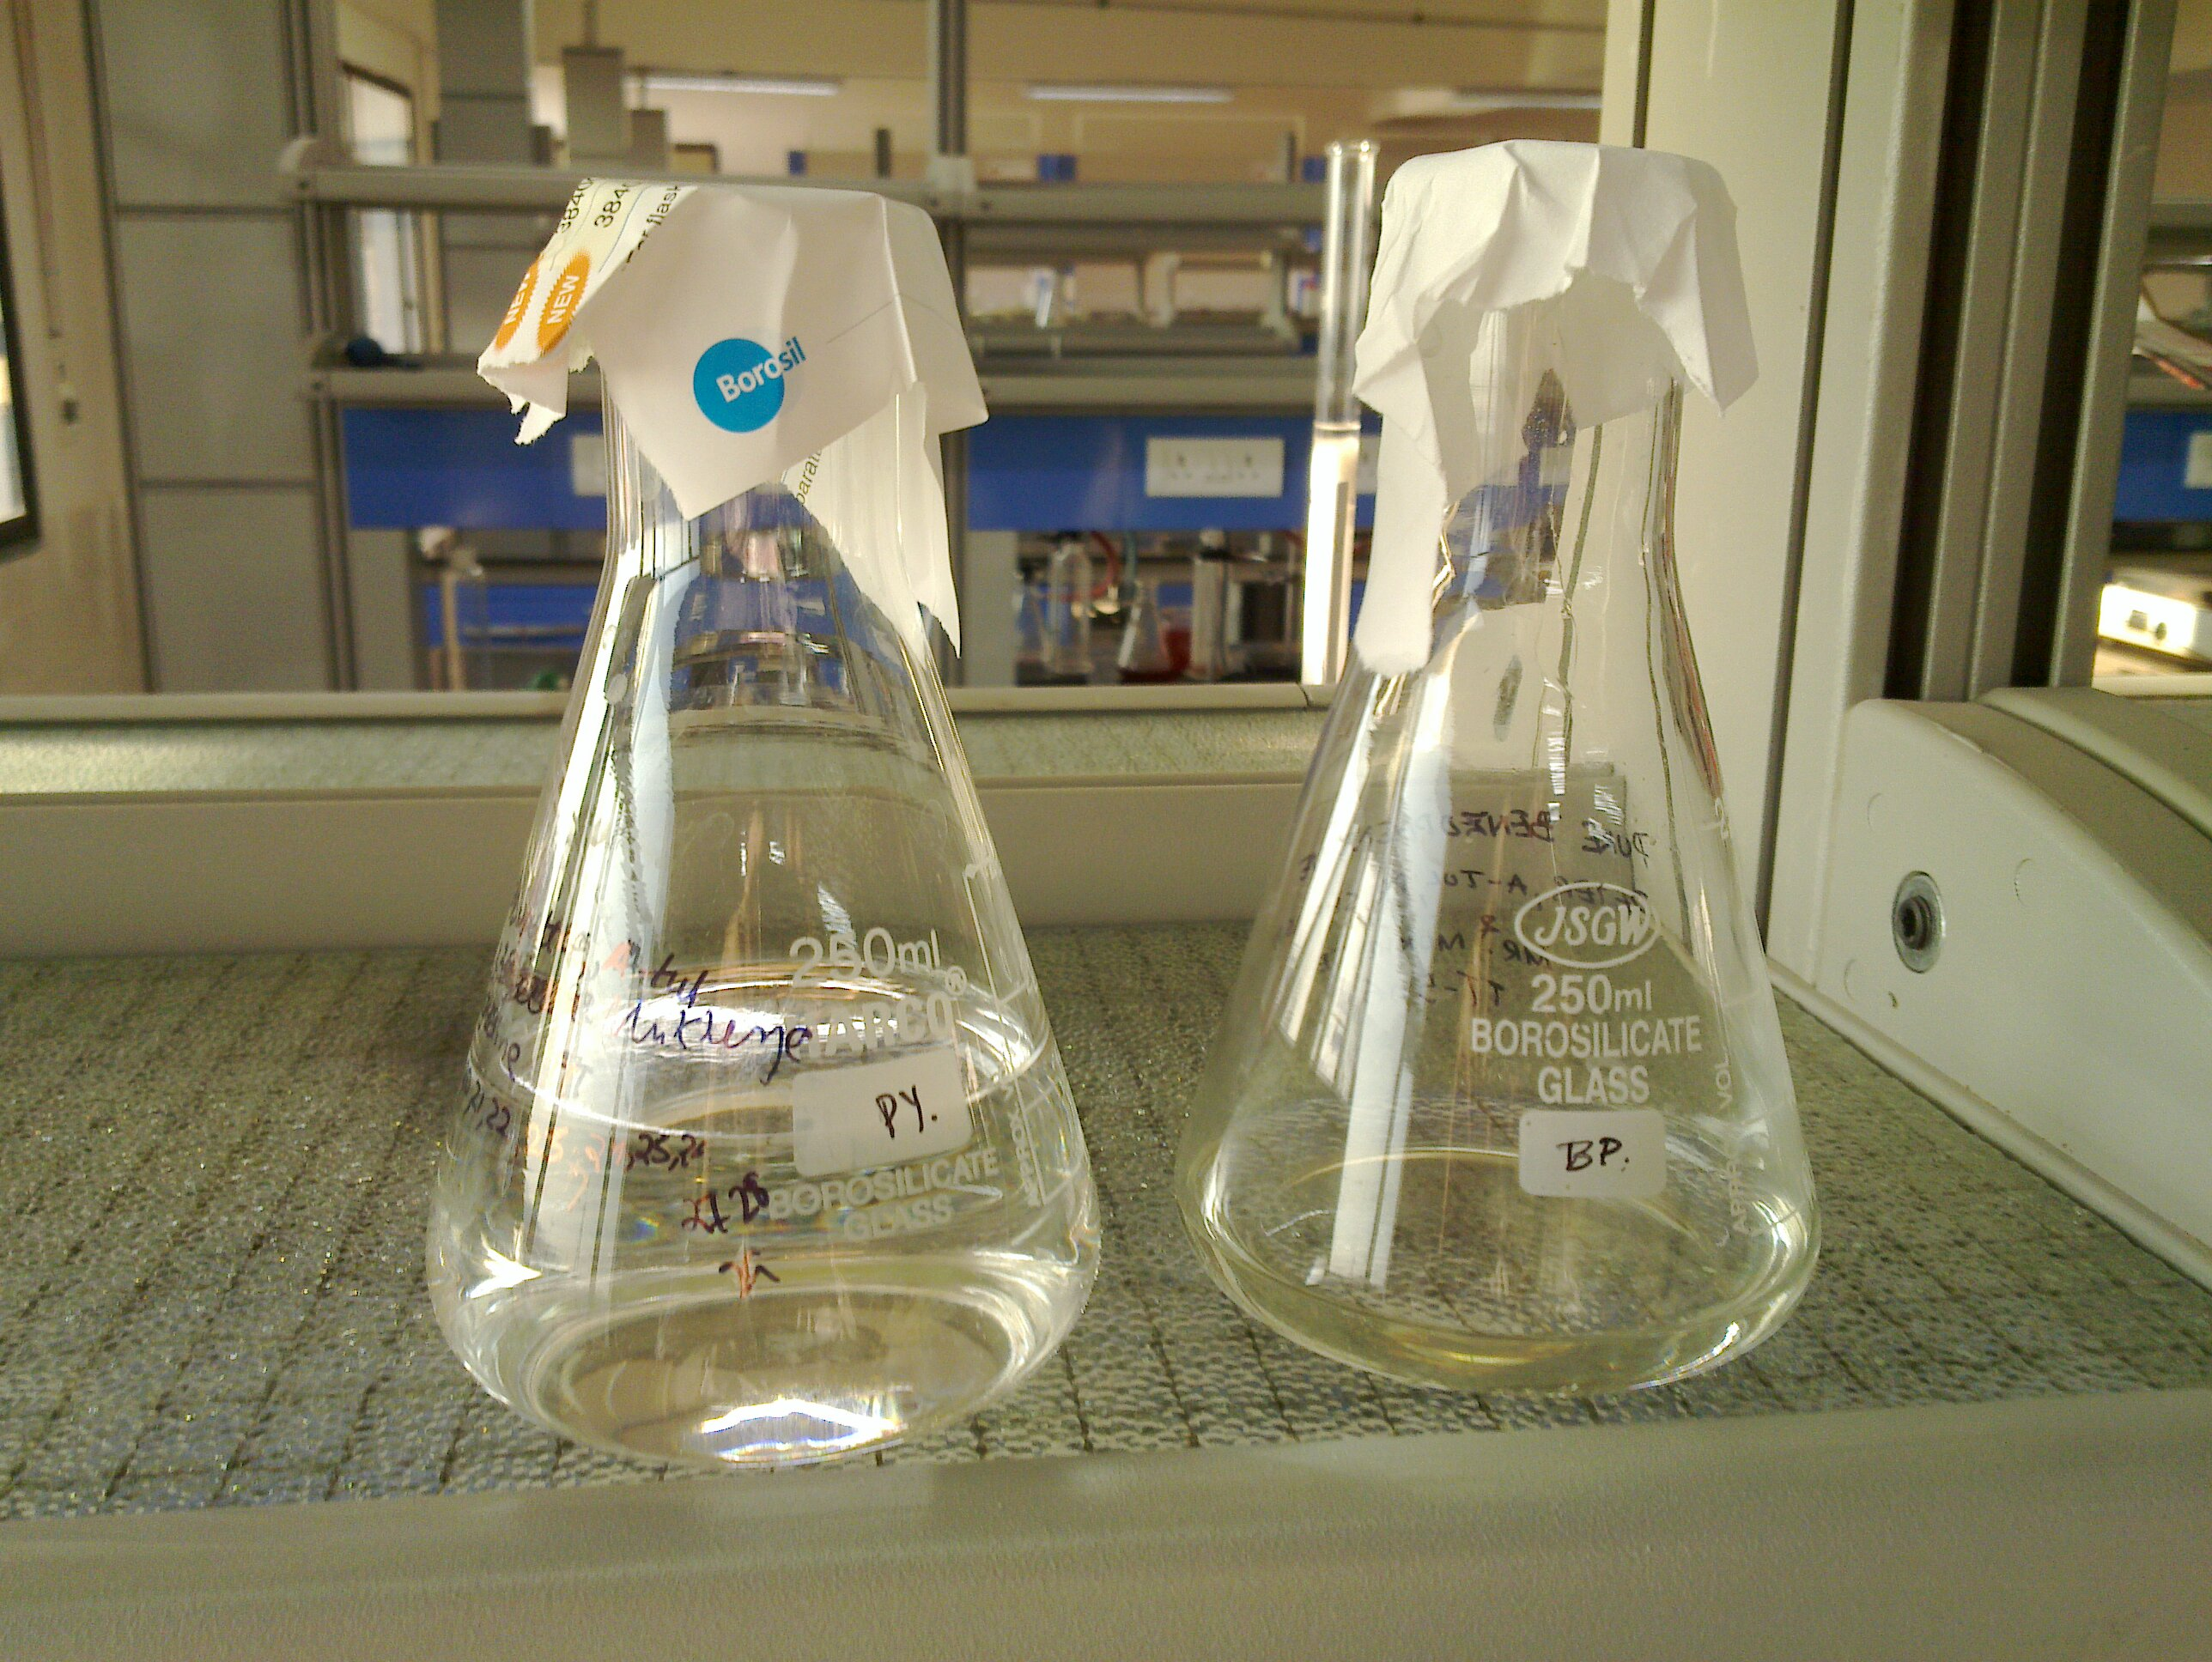
\includegraphics[width=1.2\linewidth]{gfx/e4_3}
		\end{center}
	\caption[Pyridine on the Left, Benzophenone on the Right]{\label{e4_3}}
	\end{figure}
